\begin{figure}[htbp]
\centering
\begin{tikzpicture}[font=\small]
\begin{scope}[x=.51cm,y=-.51cm]
  \fill[black!4] (0,0) rectangle (5,5);
  \fill[teal!18] (0,2) rectangle (5,3);
  \fill[teal!18] (2,0) rectangle (3,5);
  \foreach \i in {0,...,5}{
    \draw[black!48,thin] (0,\i) -- (5,\i);
    \draw[black!48,thin] (\i,0) -- (\i,5);
  }
  \foreach \i in {0,...,4}{
    \node[left] at (0,\i+.5) {\scriptsize\i};
    \node[above] at (\i+.5,0) {\scriptsize\i};
  }
  \foreach \r/\c in {0/1,1/4,3/0,4/3}{
    \fill (\c+.5,\r+.5) circle[radius=2.7pt];
  }
  \draw[teal!65!black,line width=.9pt] (2.5,2.5) circle[radius=3.1pt];
  \node[anchor=north] at (2.5,5.25) {(a) A $5\times5$ board};
\end{scope}
\begin{scope}[shift={(5.15,0)},x=2.55cm,y=-2.55cm]
  \draw[black!60] (0,0) rectangle (1,1);
  \draw[teal!65!black,thick] (0,0) -- (1,1);
  \draw[teal!65!black,thick,dashed] (0,.5) -- (.5,1);
  \node[fill=white,inner sep=1pt,font=\scriptsize] at (.61,.59) {$r-c=0$};
  \node[fill=white,inner sep=1pt,font=\scriptsize] at (.25,.77) {$r-c=\tfrac12$};
  \node[left] at (0,0) {$0$}; \node[left] at (0,1) {$1$};
  \node[above] at (1,0) {$1$};
  \node[above] at (.50,0) {column $c$};
  \node[rotate=90] at (-.20,.50) {row $r$};
  \node[anchor=north] at (.5,1.05) {(b) Unit square};
\end{scope}
\end{tikzpicture}
\caption{From the board to the lines of the unit square. In (a), each black dot represents a queen.
Row~2 and column~2 are empty. The circle marks their intersection.
In (b), each value of $r-c$ identifies a diagonal. Its projection onto the row axis has
length one for the solid line and one half for the dashed line.}
\label{fig:tablero-fibras}
\end{figure}